\documentclass[a4paper,12pt]{report}
\usepackage[margin=1in]{geometry} % to change the page dimensions
\usepackage{ctex}
\usepackage{xeCJK}
\usepackage{comment}
%\usepackage{times}
\usepackage{setspace}
% \usepackage{lastpage}
\usepackage{fancyhdr}
\usepackage{graphicx}
%\graphicspath{{fig/}}
\usepackage{wrapfig}
\usepackage{subfigure}
\usepackage{array}  
% \usepackage{fontspec,xunicode,xltxtra}
% \renewcommand{\sfdefault}{cmr}
\usepackage{titlesec}
\usepackage{titletoc}
\usepackage[titletoc]{appendix}
%\usepackage[top=30mm,bottom=30mm,left=20mm,right=20mm]{geometry}
%\usepackage{cite}
\usepackage[backend = biber, style = gb7714-2015, defernumbers=true]{biblatex}
\renewcommand*{\bibfont}{\small}
\addbibresource{reference.bib}
%\usepackage{courier}
\setmonofont{Courier New}
\usepackage{listings}
\lstset{tabsize=4, keepspaces=true,
    xleftmargin=2em,xrightmargin=0em, aboveskip=1em,
    %backgroundcolor=\color{gray!20},  % 定义背景颜色
    frame=none,                       % 表示不要边框
    extendedchars=false,              % 解决代码跨页时,章节标题,页眉等汉字不显示的问题
    numberstyle=\ttfamily,
    basicstyle=\ttfamily,
    keywordstyle=\color{blue}\bfseries,
    breakindent=10pt,
    identifierstyle=,                 % nothing happens
    commentstyle=\color{green}\small,  % 注释的设置
    morecomment=[l][\color{green}]{\#},
    numbers=left,stepnumber=1,numberstyle=\scriptsize,
    showstringspaces=false,
    showspaces=false,
    flexiblecolumns=true,
    breaklines=true, breakautoindent=true,breakindent=4em,
    escapeinside={/*@}{@*/},
}
\usepackage{amsmath}
\usepackage{amsthm}
\newtheorem{theorem}{定理}
\newtheorem{definition}{定义}
\newtheorem{corollary}{推论}
\newtheorem{example}{例}
\usepackage{amsfonts}
%\usepackage{bm}
\usepackage{booktabs} % for much better looking tables
\usepackage{paralist} % very flexible & customisable lists (eg. enumerate/itemize, etc.)
\usepackage{verbatim} % adds environment for commenting out blocks of text & for better verbatim
\usepackage{subfigure} % make it possible to include more than one captioned figure/table in a single float
% These packages are all incorporated in the memoir class to one degree or another...
\usepackage{cases} %equation set
\usepackage{multirow} %use table
\usepackage{algorithm}
\usepackage{algorithmic}
\usepackage{hyperref}
\hypersetup{colorlinks,linkcolor=black,anchorcolor=black,citecolor=black, pdfstartview=FitH,bookmarksnumbered=true,bookmarksopen=true,} % set href in tex & pdf
%\usepackage[framed,numbered,autolinebreaks,useliterate]{mcode} % 插入matlab代码
\XeTeXlinebreaklocale "zh"
\XeTeXlinebreakskip = 0pt plus 1pt minus 0.1pt

%---------------------------------------------------------------------
%	页眉页脚设置
%---------------------------------------------------------------------
\fancypagestyle{plain}{
    \pagestyle{fancy}      %改变章节首页页眉
}

\pagestyle{fancy}
\lhead{\kaishu~软件工程概论作业~}

\cfoot{\thepage}
\titleformat{\chapter}{\centering\zihao{2}\heiti}{第\chinese{chapter}章}{1em}{}
% \titleformat{\chapter*}{\centering\zihao{-1}\heiti}
\begin{comment}
%---------------------------------------------------------------------
%	章节标题设置
%---------------------------------------------------------------------
\titleformat{\chapter}{\centering\zihao{-1}\heiti}{实验\chinese{chapter}}{1em}{}
\titlespacing{\chapter}{0pt}{*0}{*6}
\end{comment}
%---------------------------------------------------------------------
%	摘要标题设置
%---------------------------------------------------------------------
%\renewcommand{\abstractname}{摘要}
\renewcommand{\figurename}{图}
\renewcommand{\tablename}{表}

%---------------------------------------------------------------------
%	参考文献设置
%---------------------------------------------------------------------
%\renewcommand{\bibname}{\zihao{2}{\hspace{\fill}参\hspace{0.5em}考\hspace{0.5em}文\hspace{0.5em}献\hspace{\fill}}}
\renewcommand{\bibname}{参考文献}
\begin{comment}
%---------------------------------------------------------------------
%	引用文献设置为上标
%---------------------------------------------------------------------
\makeatletter
\def\@cite#1#2{\textsuperscript{[{#1\if@tempswa , #2\fi}]}}
\makeatother
\end{comment}
%---------------------------------------------------------------------
%	目录页设置
%---------------------------------------------------------------------
%\renewcommand{\contentsname}{\zihao{-3} 目\quad 录}
\renewcommand{\contentsname}{目录}
\titlecontents{chapter}[0em]{\songti\zihao{-4}}{\thecontentslabel\ }{}
{\hspace{.5em}\titlerule*[4pt]{$\cdot$}\contentspage}
\titlecontents{section}[2em]{\vspace{0.1\baselineskip}\songti\zihao{-4}}{\thecontentslabel\ }{}
{\hspace{.5em}\titlerule*[4pt]{$\cdot$}\contentspage}
\titlecontents{subsection}[4em]{\vspace{0.1\baselineskip}\songti\zihao{-4}}{\thecontentslabel\ }{}
{\hspace{.5em}\titlerule*[4pt]{$\cdot$}\contentspage}

\begin{document}
%---------------------------------------------------------------------
%	封面设置
%---------------------------------------------------------------------
\begin{titlepage}
	\begin{flushleft}
    
\includegraphics[width=0.4\textwidth]{haut.png}\\
	\end{flushleft}
    \begin{center}        
    \vspace{2.5cm}
    \textbf{\zihao{0}{\heiti{软件工程概论作业}}}\\[1cm]
	\textbf{\zihao{1}{\heiti{作业1:如何提升搜索质量}}}\\
    \vspace{\fill}
    
\setlength{\extrarowheight}{3mm}
{\songti\zihao{3}	
\begin{tabular}{rl}
    
    {\makebox[4\ccwd][s]{学\qquad 号:}} & ~\kaishu 201816040209 \\
    {\makebox[4\ccwd][s]{姓\qquad 名:}} & ~\kaishu 程\quad 长 \\
    {\makebox[4\ccwd][s]{年\qquad 级:}} & ~\kaishu 2018级 \\
    {\makebox[4\ccwd][s]{专\qquad 业:}} & ~\kaishu 软件工程 \\
    {\makebox[4\ccwd][s]{授课教师:}}  & ~\kaishu 王珂\\ 
    {\makebox[4\ccwd][s]{完成日期:}}  & ~\kaishu 2020年2月5日\\ 

\end{tabular}
 }\\[2cm]
%\vspace{\fill}
%\zihao{4}
%使用\LaTeX 撰写于\today
    \end{center}	
\end{titlepage}




%---------------------------------------------------------------------
%  目录页
%---------------------------------------------------------------------
\tableofcontents % 生成目录

%---------------------------------------------------------------------
%  实验目的
%---------------------------------------------------------------------
\chapter{问题1}
\setcounter{page}{1}

\section{搜索质量的差异}

\begin{center}%居中格式
    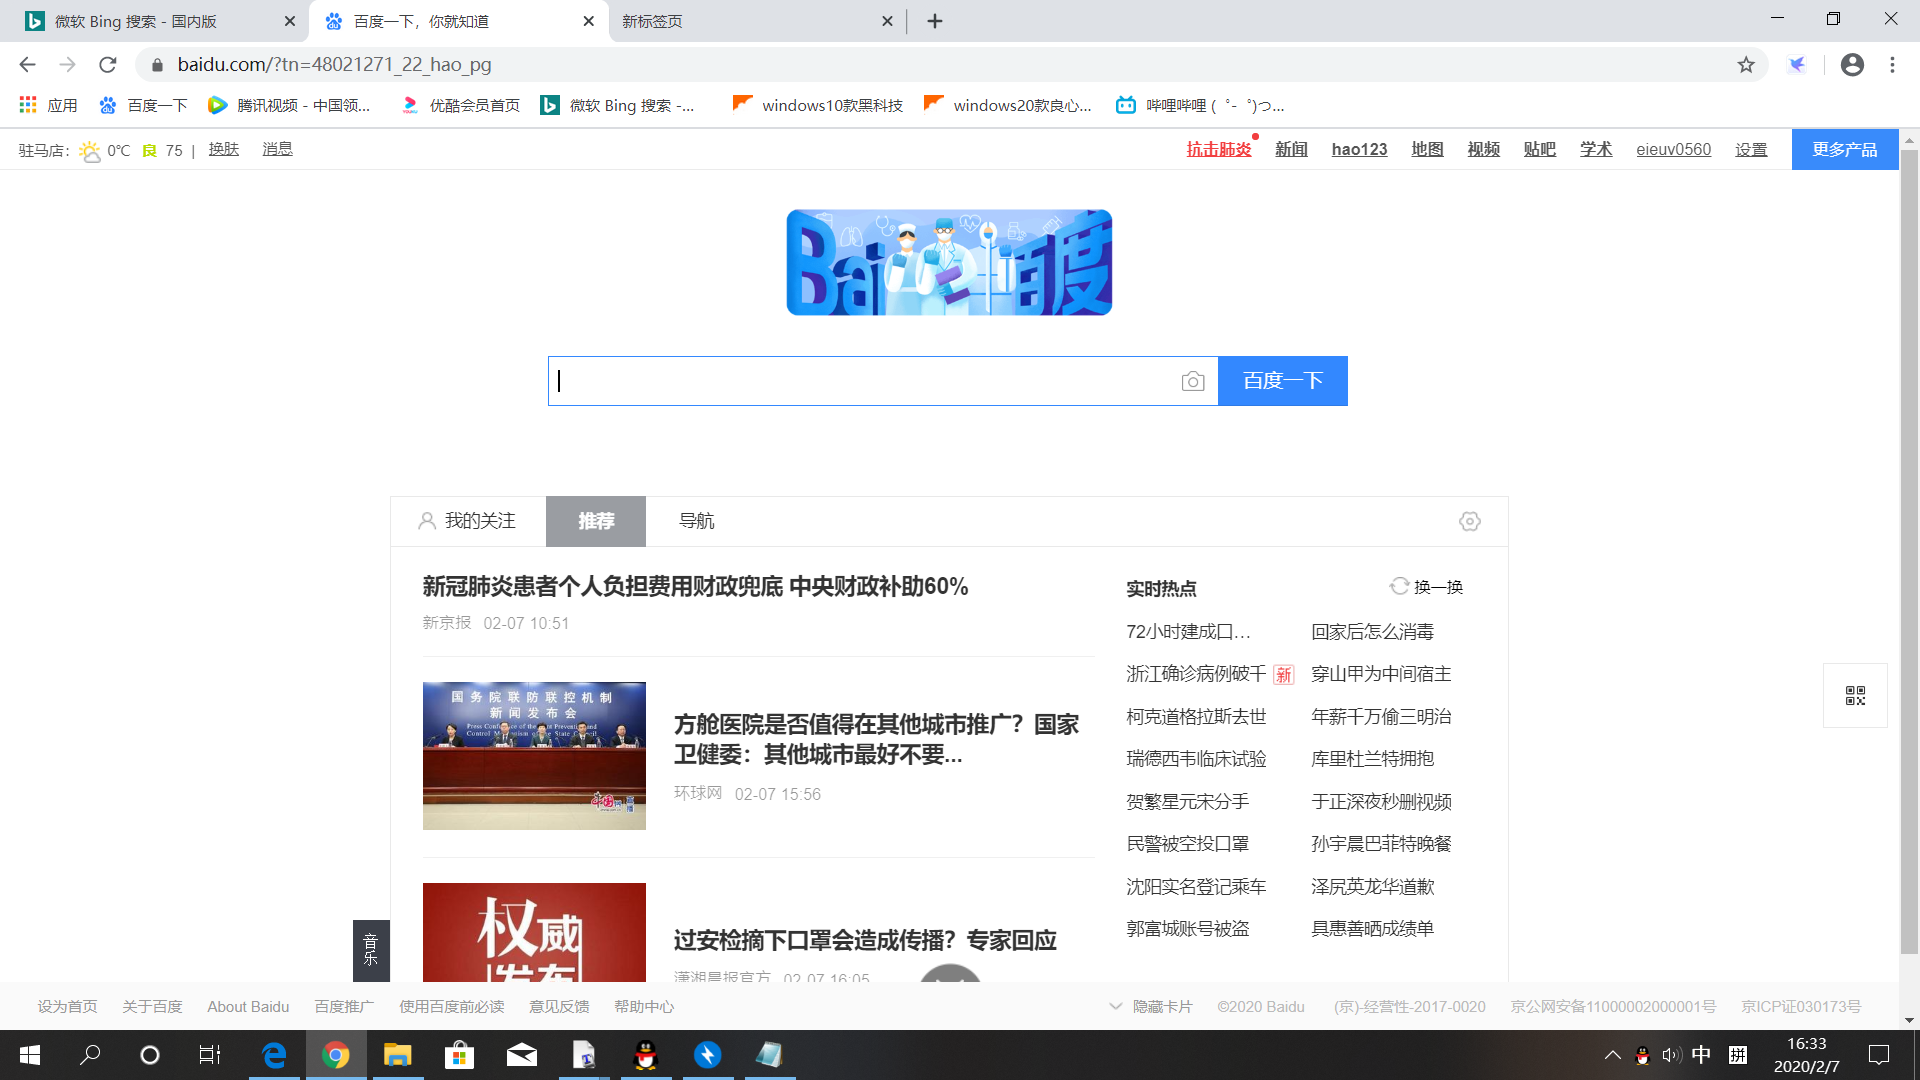
\includegraphics[width=0.5\textwidth]{baidu.png} %左边的图
\end{center}

\begin{center}%居中格式
    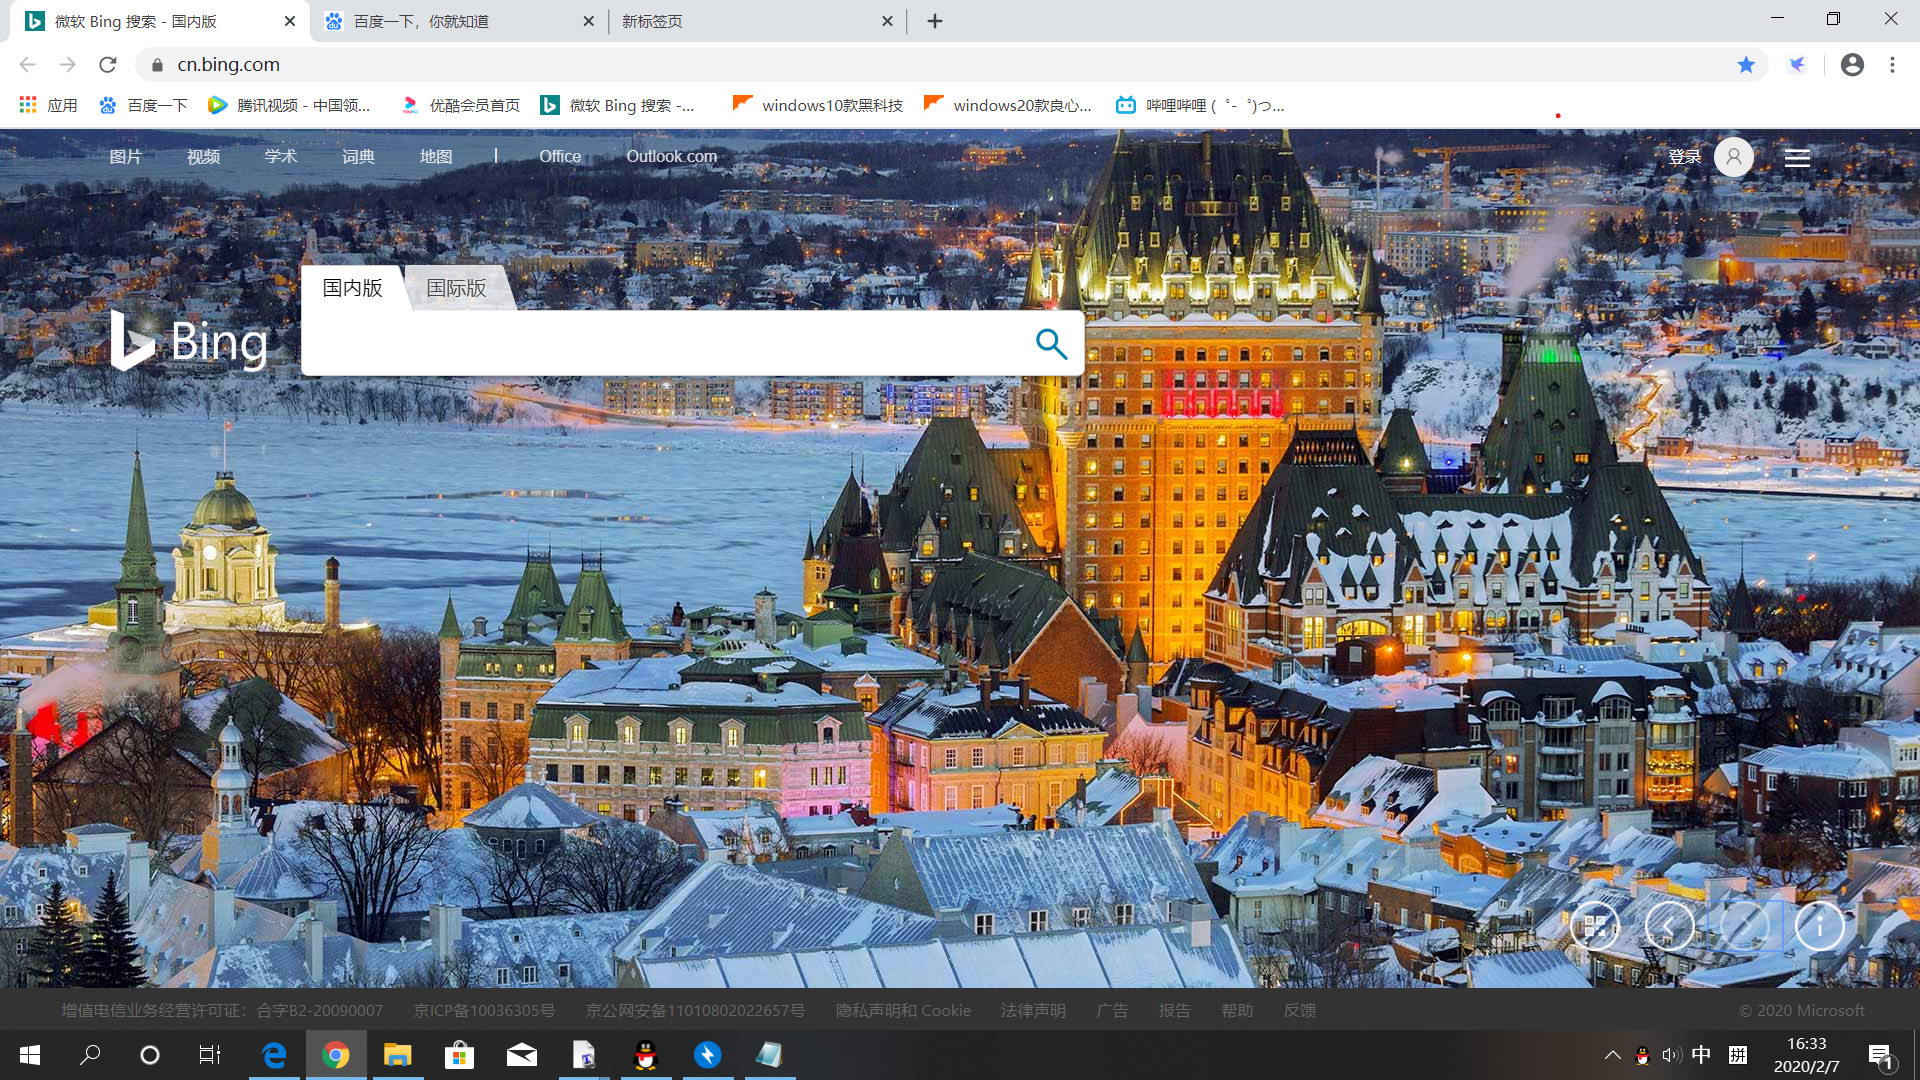
\includegraphics[width=0.5\textwidth]{bing.png} %左边的图
\end{center}

\begin{center}%居中格式
    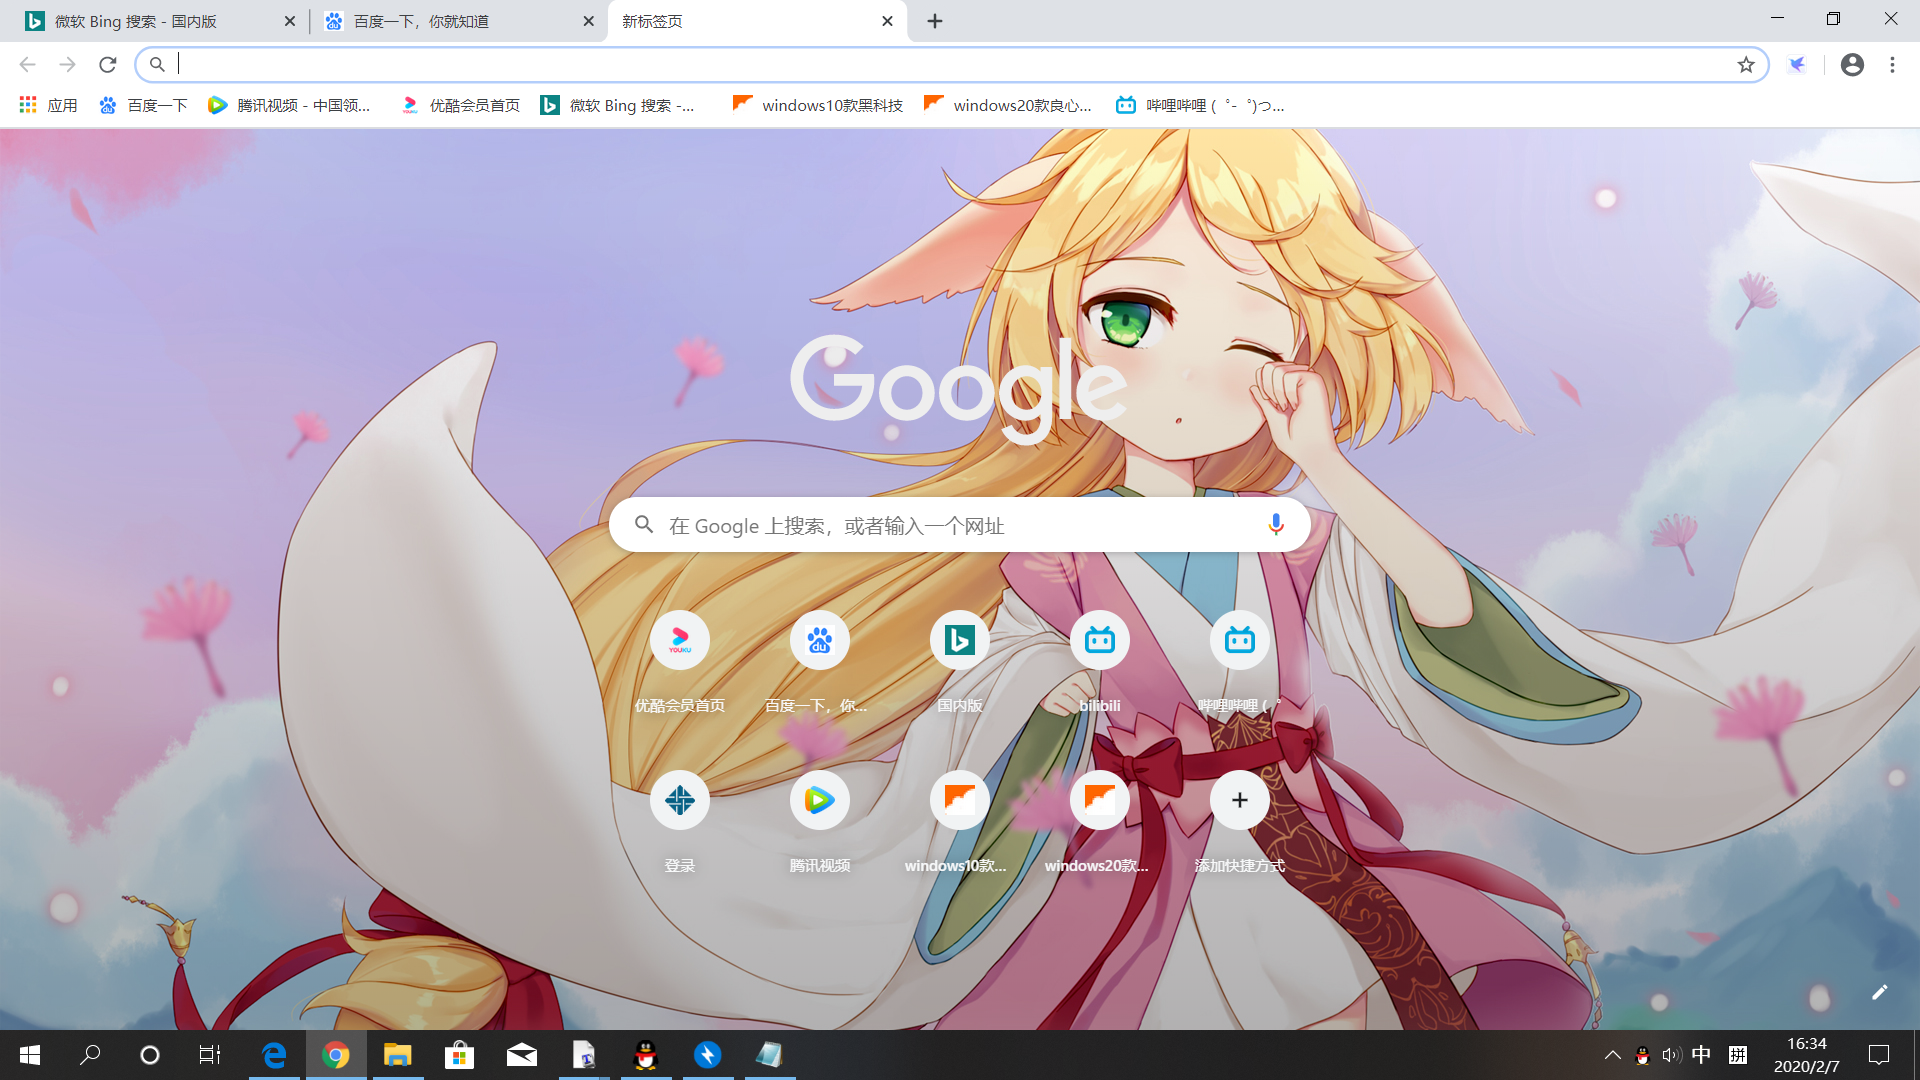
\includegraphics[width=0.5\textwidth]{Goole.png} %左边的图
\end{center}

\begin{itemize}
    \item 
从搜索界面上来看,必应背景图更好看,之前Goole和百度都是白色背景图(现在百度和Goole支持自定义背景图),必应的背景图会每日更换,有图片索引支持查看图片中的资料,也可以切换回之前的图片,百度主页面搜索框下是新闻,Goole搜索框下面是常用网页的链接,Bing搜索框下面则什么都没有,它们都有菜单栏
\end{itemize}



\begin{center}%居中格式
    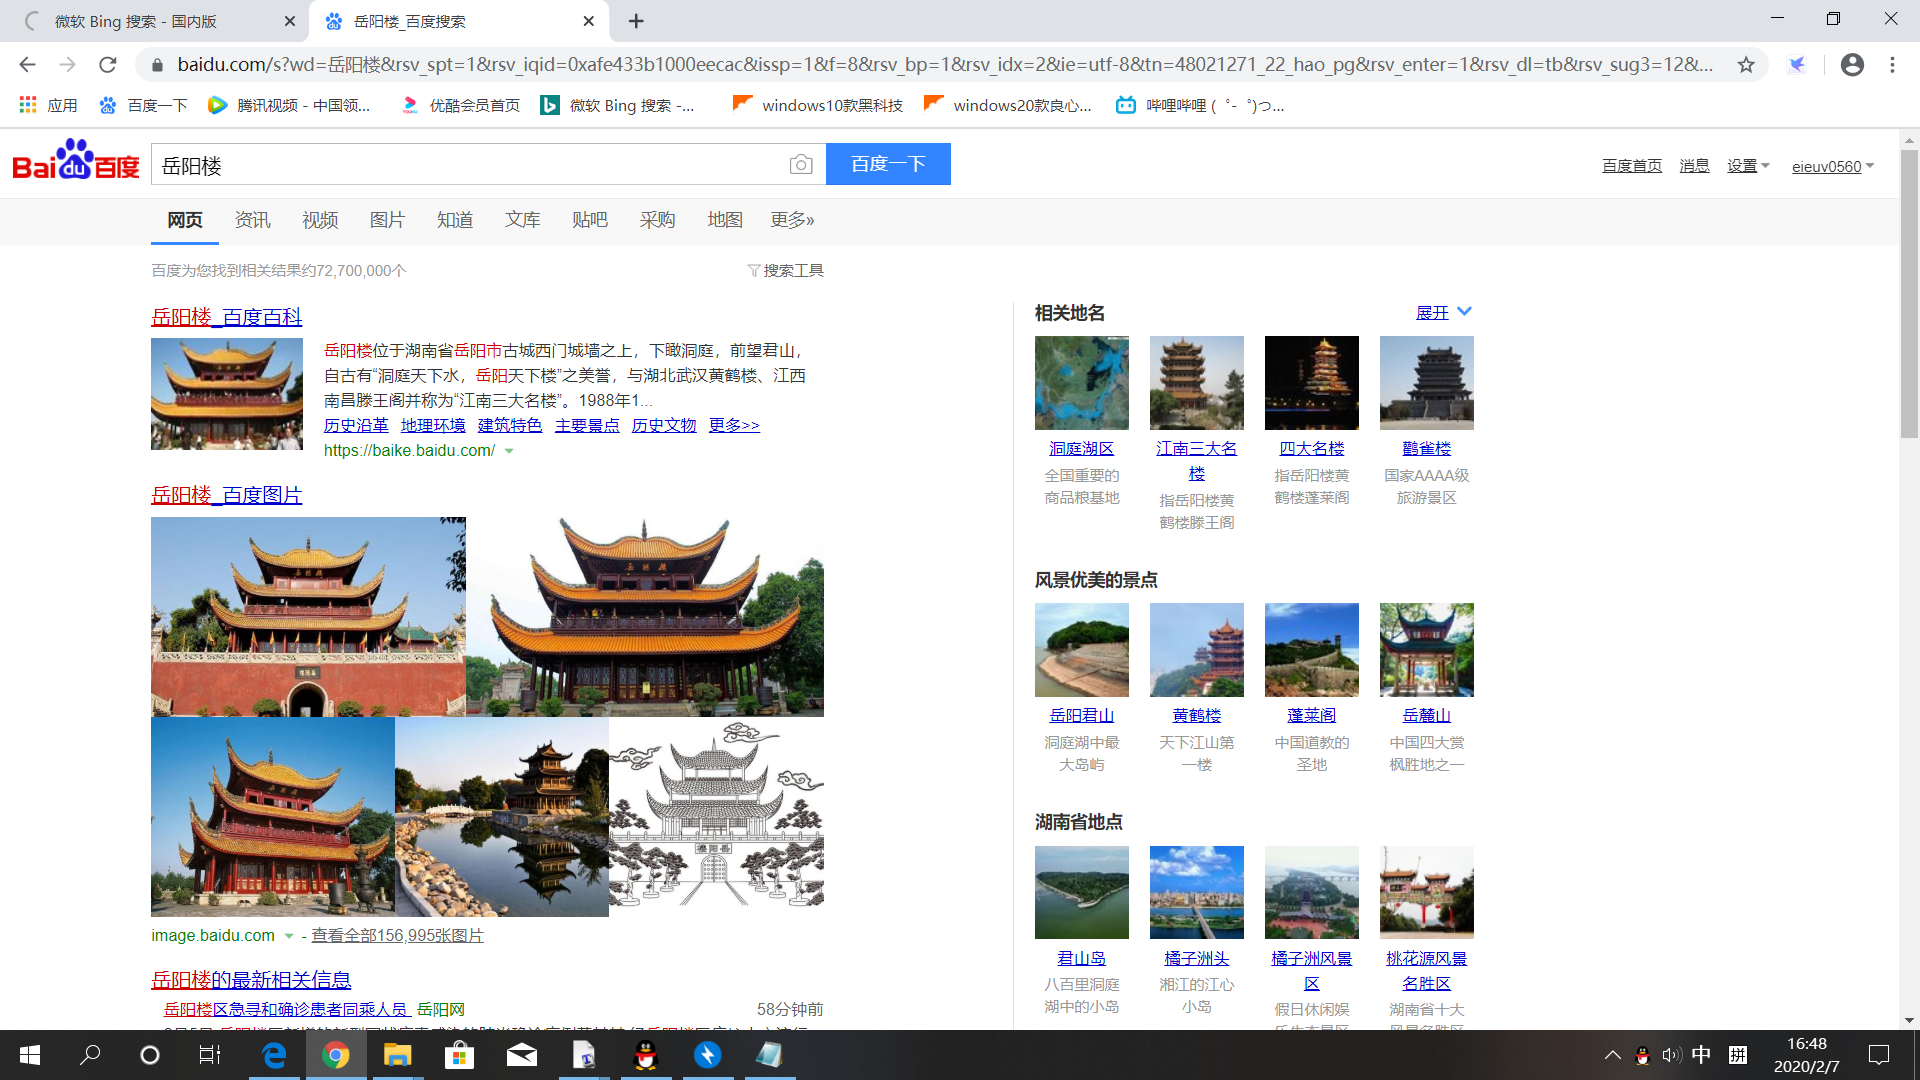
\includegraphics[width=0.5\textwidth]{1.png} %左边的图
    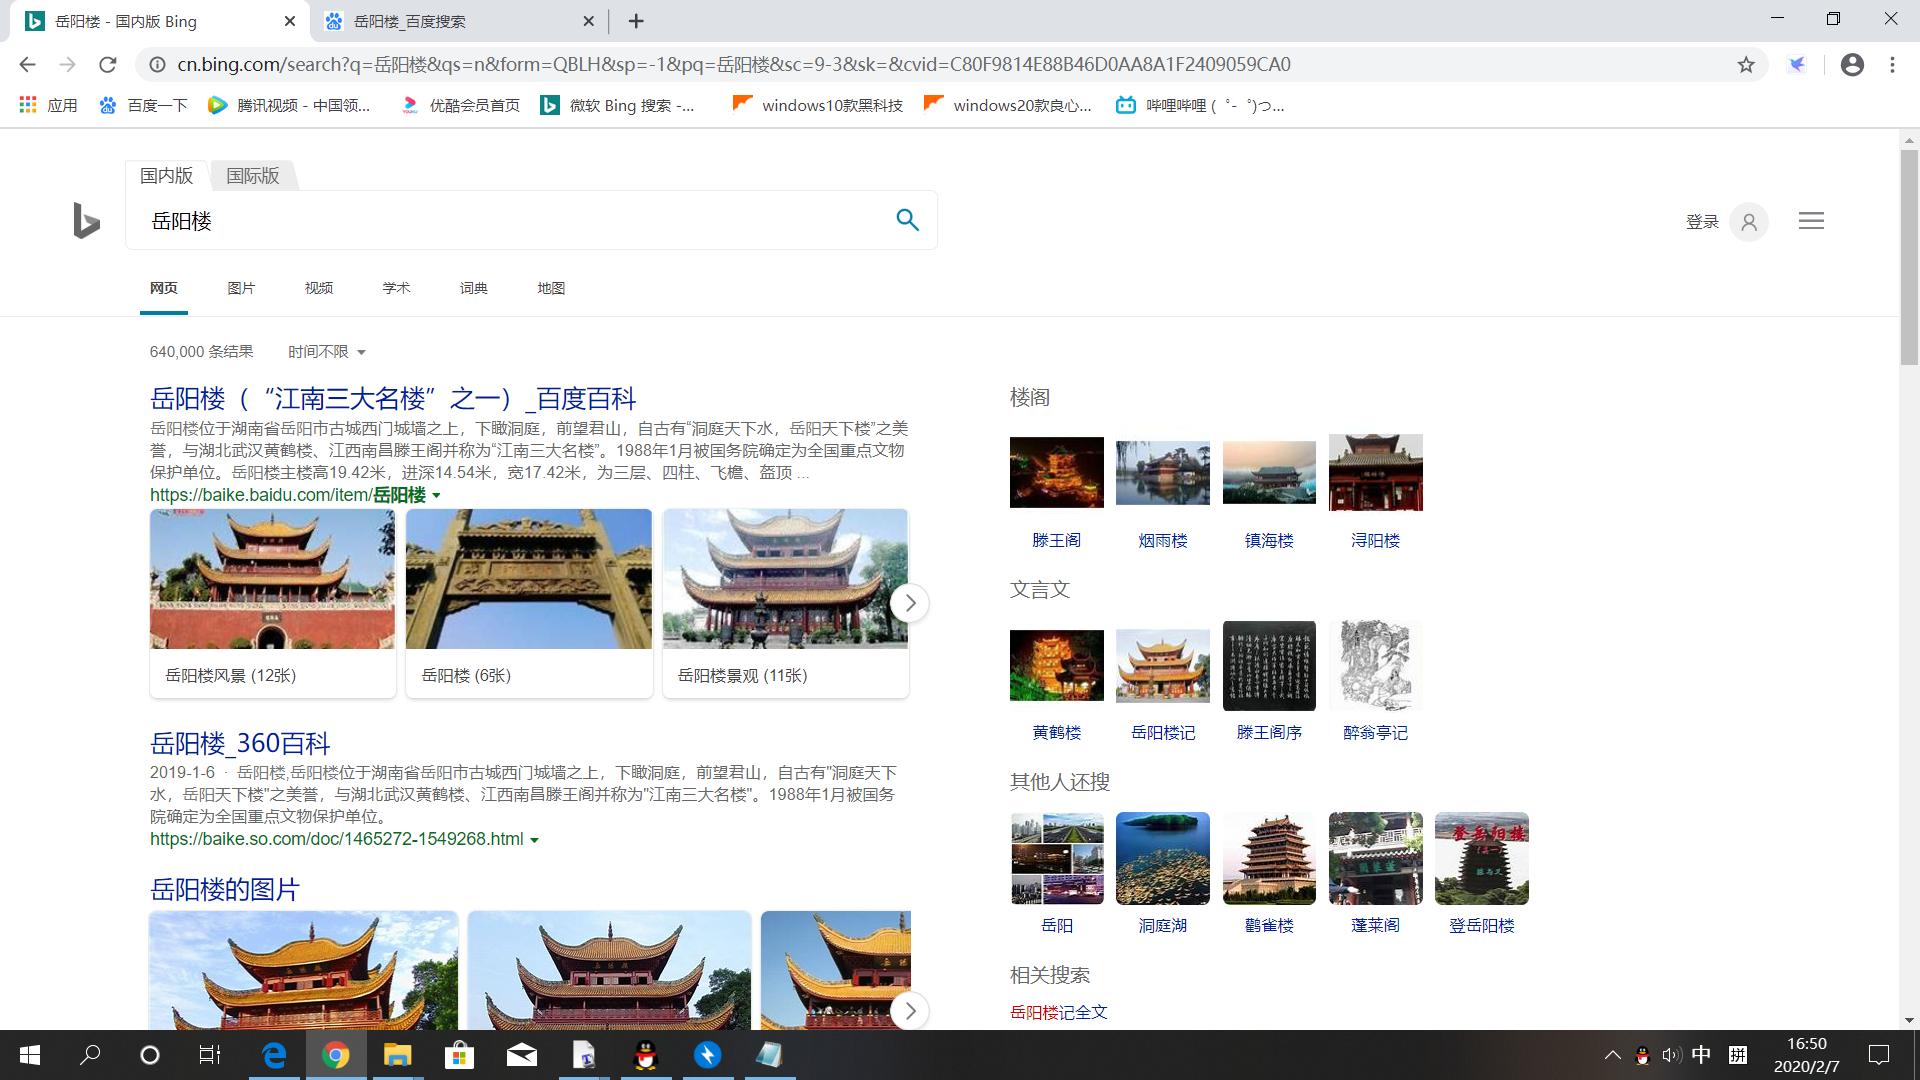
\includegraphics[width=0.5\textwidth]{2.png} %左边的图
\end{center}

\begin{itemize}
    \item 
从搜索内容上看、对于绝大多数网站,此项指标当属谷歌老大,收录量有时甚至是其他搜索引擎的好几倍,下来排名:谷歌>百度>必应。例如搜索岳阳楼百度前2条是直接与岳阳楼相关的内容,必应的前4条都是与岳阳楼直接相关的内容,必应和百度搜索最下面是岳阳楼的相关搜索,百度的右侧显示的是相关地名,景点,地点,以及一个热搜榜单,Bing右侧显示相关搜索,楼阁,文言文,以及其他人搜索。个人认为必应的质量比百度高,但是百度的收录量很大,有些编程方面的文章百度搜到的更全面
\end{itemize}


\begin{itemize}
    \item 
如果以搜索结果精准度来说,三家的排位是谷歌、必应、百度。谷歌在搜索结果内容上是最好的,多年搜索域名的开发经验加上强大的技术优势,谷歌在搜索结果上居于全球领先地位。必应的众多优势在于微软拥有自己的内容提供公司。采用的是Powerset技术(Powerset是微软收购的一家搜索技术公司)。是微软借以取代原有的Live Search的新一代搜索引擎,但现在毕竟是刚开始,各个方面不是太完善,个人认为现在跟谷歌和百度比,还是稍差一点。百度是全球最大的中文搜索引擎,在中国居于霸主地位,更贴近中国客户的使用感受,在中文内容(音乐、视频、娱乐、图片等)方面有着先天优势,用起来更符合中国人的使用习惯,但个人认为在搜索内容和结果方面稍逊一筹。 
\end{itemize}

%---------------------------------------------------------------------
%  示例1
%---------------------------------------------------------------------
\chapter{问题2} 

\section{如何进行高质量的搜索}


\begin{itemize}
    \item 
 1,搜索引擎 搜索引擎的选择对于搜索结果的影响是最为关键的。综合性的搜索引擎(比如百度谷歌)能解决日常搜索百分之80的情况(二八定律),想要更快速的得到结果,你就要使用细分的搜索引擎,比如搜索英文资料时,你应该用”Google No Country Redirect“搜索,而不是”谷歌“搜索,搜索问题解答时,你应该用”百度知道“搜索,而不是”百度“搜索。剩下的那更具搜索价值那百分之20内容,你就要使用专业的搜索引擎,它不仅更快,而且也能搜索到综合性引擎搜索不到的内容。比如搜索最新鲜的资讯你需要用”微博“搜索引擎,论文搜索你要用”文献“搜索引擎,图片搜索你需要用专业的图片搜索引擎等。 
\end{itemize}

\begin{itemize}
    \item 
2,搜索表达式 很多用户都还是停留在搜索框中输入一两个关键字,然后点击搜索按钮的阶段,这是非常低效和无用的。运气好你可以在第一页就得到结果,否则你需要不停的翻页来得到结果,学习一些搜索引擎常用的检索表达式是一件低投入高回报,受益终身的事情。而且搜索表达式在绝大多数引擎上都是适用的。 检索表达式介绍示例-搜索关键词A的同时屏蔽关于关键词B的信息apple -iphone|同时搜索关键词多个关键词, |可以用OR代替, OR需要大写apple|google, apple OR google""要求查询结果要精确匹配,不包括演变形式"Failure is the mother of success"*只适用于英文,添加一个星号以表示任何未知或不确定的字词。"* is the mother of success"《》只适用于中文,要求查询结果是关于这部作品,而不是普通的词语《Baby》site:仅从特定网站或网域获得搜索结果site:qq.cominurl:查找在URL地址里有搜索关键词的页面inurl:qqintitle:查找在网页标题里有搜索关键词的页面intitle:qqfiletype:查找pdf,xml,xls,txt,doc,csv等特定格式的结果filetype:pdf qq混合搜索同时使用多个检索表达式,比如:site:qq.com "firefox" -quantum 
\end{itemize}

\begin{itemize}
    \item 
3,筛选结果 搜索结果筛选的使用可以加速获得搜索结果,不要只是在逛淘宝时才用到搜索筛选,比如搜索视频是按播放次数最多排列,搜索答案时按最多点赞排列,新闻搜索时按最新发布排列,还可以筛选某一个时间阶段的内容。 
\end{itemize}

\begin{itemize}
    \item 
4,选择结果 在得到比较满意的搜索结果时,你可以按住 Ctrl 键点击搜索结果就会在新的标签页面打开,方便对比结果。如果点击的链接,因为一些原因打不开了,可以利用“网页快照”的功能来重新查看。如果想要知道这个网页的旧版本,可以使用”互联网档案馆“(Internet Archive)来查看。当搜索结果不完整或者不是最开始的资料来源时,可以选择其中的一串文字来重新搜索(10个汉字或者英文单词),在这一串文字的两端最好加上双引号(“”),这样能够更精准的匹配。
\end{itemize}

\end{document}